A correctly defined model, either by training or by expertise, is used to make predictions about the unobserved data in a process called inference. There are two most popular approaches to this task named marginal and maximum a posteriori (MAP) inference. Marginal inference is aimed to compute marginal distributions, which give a probability of a variable taking a given value as opposed to every other possibility. An example of it would be to segment an image into foreground and background, where one object is considered foreground and all other objects are assigned as background. On the other hand, the goal of MAP inference is to find the most probable configuration of unobserved variables’ values basing on the values of observed data. Both types of inferences are used in factor graphs and consist of establishing observed data and finding such values of output variables that minimise the total energy. In the thesis for the task of minimising the energy MAP inference was used. The reason behind this choice is that MAP inference outputs directly a state $y^* \in \pazocal{Y}$ that has the maximal probability of occurrence given an underlying factor graph, observation $x$, and learned weight vector $w$ and this is the goal of semantic image segmentation. 

State $y^*$ represents the most optimal configuration of pixel labels for a given image. Finding the optimal state would require calculating energy for each possible configuration of outputs, which is too computationally demanding to be performed. However, there are methods to provide the final result without a need of extensive calculations. Two most popular types of methods that are used for inference are Monte Carlo methods and variational algorithms \cite{crf_sutton}. Monte Carlo algorithms are a type of stochastic algorithms which instead of estimating conditional probability distributions for a given test object, base the approximation on a repetitive generation of random samples from a distribution of interest. The idea is that given an enough number of samples their mean will approximate the desired output. On the other hand, variational algorithms are aimed to find a single configuration that is an estimation of a most probable output by changing inference into an optimisation problem. Though Monte Carlo methods are more accurate with a large number of iterations they will converge to the real result, variational algorithms tend to be much faster. 

One of the most popular approaches towards variational inference in probabilistic graphical models is named Belief Propagation. It is an iterative framework based on message passing that exchange data between variable and factor nodes \cite{markov_blake}. Those messages, also named beliefs, are vectors that can be understood as a measure of certainty of related nodes that other nodes belong to some state. It is based on a concept of dynamic programming, which instead of doing calculations for each factor independently uses a recursive procedure to propagate beliefs throughout the whole graph. Recursive nature reduces the number of computations because of reusing previously computed data. Belief Propagation was first used to find exact marginals on tree \cite{bayes_pearl}, tough it is also applicable in a general case of graphs that may contain loops, however, without a guarantee of finding a global optimum. This method is applicable to both of the previously mentioned inference problems. Sum-product algorithm is used for computing marginal distribution, and max-product algorithm for solving MAP inference. 

\subsection{Sum-Product algorithm}
The sum-product algorithm is a method used to compute marginal distributions of a given test sample and a normalising constant $Z$ with the use of a trained model. Those outcomes can be described by formulae \ref{eq:sum_product_prob} and \ref{eq:sum_product_z}.
\begin{equation}
    \label{eq:sum_product_prob}
    p(y|x,w)=\frac{1}{Z}\exp{\bigg(-\sum_{f \in \pazocal{F}}{E_f(y_f)}\bigg)} 
\end{equation}
\begin{equation}
    \label{eq:sum_product_z}
     Z=\sum_{y \in \pazocal{Y}}{\exp{\bigg(-\sum_{f \in \pazocal{F}}{E_f(y_f)}\bigg)}} 
\end{equation}

In the Sum-Product algorithm, factor energy can be computed based on information sent from adjacent nodes in a form of messages, which are aimed to propagate observed data throughout the whole model. They are sent through each edge of a factor graph in both directions. The messages sent from variable nodes to factors are denoted as $q_{Y_i\rightarrow F}$ and factor-to-variable message can be expressed as $r_{F\rightarrow Y_i}$, where $Y_i$ denotes an $i^{th}$ variable node \cite{Nowozin}. Variable-to-factor messages depend on previously calculated factor-to-variable messages that are associated with factors adjacent to the given variable. They can be formulated as a summation of messages from each factor $F'$ from the variable neighbourhood $M$ with an exception of the factor $F$ to which the initial message is directed. Such a belief is then calculated for each variable node $i$ and for every label $y$ from the output domain of a given problem as in formula \ref{eq:belief_q_1}.
\begin{equation}
    \label{eq:belief_q_1}
    q_{Y_i\rightarrow F}(y_i)=\sum_{F' \in M(i) \setminus \left \{ F \right \} }{ r_{F'\rightarrow Y_i}(y_i)}
\end{equation}

Similarly, when it comes to computing messages from factors to variables there is a summation of messages from each variable j from the neighbourhood $N$ of the factor $F$ apart from a variable $i$ which is a recipient of the initial message. Furthermore, factor-to-variable messages take into consideration factor potentials expressed in terms of energy. These messages are again calculated for every label $y$ separately. Given the fact that one component of factor energy is a pairwise potential, which is dependent on labels of every variable connected to the factor, while computing these messages there is an extra summation over all possible states of neighbouring variables. This is needed to calculate energy for every factor state $y'_F$. This state can be understood as a label configuration of variables adjacent to the factor knowing that the variable to which the message is directed has been labelled with $y$. A formula for a factor-to-variable message is presented below. 
\begin{equation}
    r_{F\rightarrow Y_i}(y_i) = \log{\bigg(
        \sum_{\substack{{y'}_{F}\in \pazocal{Y}_F                              \\ {y'}_i = y_i}}
        \exp{\Big(-{E_F}({y'}_F) +
        \sum_{j \in N (F) \setminus \left \{ i \right \}}
            {q_{Y_j\rightarrow F}({y'}_j)}
    \Big)} \bigg)}
\end{equation}

Both of those kinds of messages are depended on previous computations, however, for trees, there are two situations in which they can be calculated without prior knowledge. For leaf nodes that are only connected to one factor, a variable-to-factor message will be equal to 0, as the neighbourhood $M(i)\setminus{\left \{ F \right \}}$ will have no elements. Message from factor to variables can be also calculated for factors that are only connected to one variable. In such a situation neighbourhood $N(F)\setminus{\left \{ i \right \}}$ will have 0 elements and consequently only an energy term is needed for the message to be calculated. If a graph contains no cycles, using those calculated beliefs recursively other messages can be computed \cite{lbp}. For tree-like structures, message computations start with choosing an arbitrary node as a root node. Then, there is a two-step procedure, which is forward and backward propagation of beliefs. Initially, starting from leaf nodes, messages are computed and passed to the root node. They are then are transferred from every node to their parents after all the messages from the node’s children are received. They carry information about an optimal label of the root node. After all messages are computed the propagation starts again but in reverse direction, which is from the root to all leaves. In this step, optimal labels for all non-root nodes are predicted. In those two steps, messages of every edge of the tree-like graph are established and can be used to calculate marginals. Then, for every variable node marginals can be computed based on factor-to-variable messages from all adjacent factors. Again, normalisation with a partition function $Z$ is needed for the marginals to carry probabilistic information. It is defined based on the summation of factor-to-variable messages directed towards the root node $r$ for every possible label $y$. Formulae below are used to compute both marginals and their normalising constant.
\begin{align}
    p(y_i) &= \exp{\bigg(\sum_{F \in M(i)}{r_{F\rightarrow Y_i}(y_i)} - \log{Z}\bigg)} \\
    \log{Z} &= \log{\sum_{y_r \in \pazocal{Y}_r}{
         \exp{\bigg(\sum_{F \in (r)}{r_{F\rightarrow Y_r}(y_r)}\bigg)
     }}}
\end{align}
To obtain a final result, which is the most probable configuration of labels for a set of variables $i \in V$ it is enough to calculate marginals for each variable and every possible label $y$ and to chose the one with the highest probability.

Tough Belief Propagation was designed to be used for non-cyclic, tree-like structures it is also possible to apply its concepts to the general case of graphs that may contain cycles, which are the most common type in computer vision tasks \cite{lbp_byung}. With graphs that contain loops it is impossible to determine a root node, hence, a previously stated algorithm for exact determination of marginals is inapplicable, however, it can be modified to allow approximating marginals for undirected graphs, which is also a case of Conditional Random Fields. In this algorithm, named Loopy Belief Propagation, messages are first initialised with random variables and then iteratively updated until they converge. This method is based on a concept that the local neighbourhood of nodes can be viewed as a tree, and as a result, message passing algorithms are applicable to it. A transfer of those messages can be done in parallel or in a sequential scheme, in a random or predefined order \cite{MRFSurvey}. For parallel processing, computation of messages for every edge is done simultaneously and after that, they are propagated to neighbours. A sequential scheme is more similar to the original Belief Propagation method as initially messages for one node are computed and then propagated to neighbouring nodes and used for further computations. Though formula for factor-to-variable message $r_{F\rightarrow Y_i}$ is the same as in an original algorithm, the equation for messages from variable to factors is modified to contain a normalising factor as in \ref{eq:variable_factor_undirected}.
\begin{align}
    \label{eq:variable_factor_undirected}
    \bar{q}_{Y_i\rightarrow F}(y_i) &= \sum_{F' \in M(i) \setminus \left \{ F \right \} }{ r_{F' \rightarrow Y_i}(y_i)} \\
    \delta &= \log{\sum_{y_i \in \pazocal{Y}_i}{\exp{( \bar{q}_{Y_i\rightarrow F}(y_i)})}} \\
    q_{Y_i\rightarrow F}(y_i) &= \bar{q}_{Y_i\rightarrow F}(y_i) - \delta
\end{align}

In Loopy Belief Propagation the exact marginal distribution is not known, however, it is possible to compute approximate marginals. Furthermore, as in this algorithm a notion of a root node does not exist it is not possible to calculate the exact partition function. That is why local normalising constants are used. The final equation for approximate marginals is also normalised according to formulae presented below.
\begin{align}
    \bar{\mu}_i (y_i) &= \sum_{F' \in M(i)}{r_{F'\rightarrow Y_i}(y_i)} \\
    z_i &= \log{\sum_{y_i \in \pazocal{Y}_i}{\exp{( \bar{\mu}_i (y_i))}}} \\
   \mu_i (y_i) &= \exp{(\bar{\mu}_i (y_i) - z_i)}
\end{align}

Using the presented method of loopy message propagation it is possible to find the most probable label for each node of a factor graph even for non-tree-like structures. 

\subsection{Max-Product algorithm }

Finding the most probable label for each node individually may not result in the most optimal label configuration of the whole structure. MAP inference, with an example of Max-Product algorithm of Belief Propagation, addresses this problem. It is similar to the Sum-Product algorithm, as it is also based on message propagation between nodes and is exact for trees and gives an approximate result for general graphs. When the Max-Product algorithm is transformed to logarithmic space by using energies instead of factor potentials it is called a Max-Sum algorithm, or a Min-Sum if the problem is expressed as a negative log-likelihood. The difference between those algorithms and the Sum-Product method lies in the computation of factor-to-variable messages as instead of marginalisation, a maximisation over factor states for Max-Sum, or minimisation for Min-Sum variant, is performed. For Max-Sum inference, the formula for messages from a factor to a variable can be presented as in formula \ref{eq:factor_to_variable_max_product}.
\begin{equation}
    \label{eq:factor_to_variable_max_product}
   r_{F \rightarrow Y_i}(y_i) = 
       \max_{\substack{{y'}_{F}\in \pazocal{Y}_F                               \\ {y'}_i = y_i}}
       {\bigg(-E_F({y'}_F) + \sum_{j \in N (F) \setminus \left \{ i \right \}}
            {q_{Y_j\rightarrow F}({y'}_j)}\bigg)}
\end{equation}
Similarly, in a Min-Sum variant of this algorithm, factor-to-variable messages can be computes as in equation \ref{eq:min_sum_r}.
\begin{equation}
    \label{eq:min_sum_r}
   r_{F \rightarrow Y_i}(y_i) = 
       \min_{\substack{{y'}_{F}\in \pazocal{Y}_F                               \\ {y'}_i = y_i}}
       {\bigg(E_F({y'}_F) + \sum_{j \in N (F) \setminus \left \{ i \right \}}
            {q_{Y_j\rightarrow F}({y'}_j)}\bigg)}
\end{equation}

When it comes to computations of variable-to-factor message the only difference is in a formulation of normalising factor, which instead of computing logarithm of a sum of messages in exponential form, takes the average value of those messages just like in formulae below.
\begin{align}
    \bar{q}_{Y_i\rightarrow F}(y_i) &= \sum_{F' \in M(i) \setminus \left \{ F \right \} }{ r_{F' \rightarrow Y_i}(y_i)} \\
    \delta &= \frac{1}{\left |\pazocal{Y}_i \right |}{\sum_{y_i \in \pazocal{Y}_i}{\bar{q}_{Y_i\rightarrow F}(y_i)}} \\
    q_{Y_i\rightarrow F}(y_i) &= \bar{q}_{Y_i\rightarrow F}(y_i) - \delta
\end{align}

Computing of all messages for every edge of the graph allows finding such a configuration of labels, which has the highest probability of occurrence. The optimal prediction $y^*$ is obtained by determining a state that has the maximal belief for every variable, which is equivalent to finding the state of lowest energy:
\begin{equation}
   y_{i}^{*} = \argmax_{y_i \in \pazocal{Y}_i}{\mu_i (y_i)}
\end{equation}
\begin{equation}
   \mu_i (y_i) = \sum_{F' \in M(i)}{ r_{F' \rightarrow Y_i}(y_i)}
\end{equation}

\subsection{Optimal labelling prediction}

Inference is a message passing algorithm which is conducted iteratively. Initially, all variable-to-factor messages are set to 0 and because of that factor-to-variable messages can be computed. In the first iteration, those messages are calculated basing on the energy of the factors only. Then, variable-to-factor messages can be computed. This process is exactly the same for factor graphs composed of two types of nodes, which is the case in Conditional Random Fields. Figure \ref{fig:inference_msgs} depicts both kinds of messages for a factor graph constructed on an image that is to be segmented.
\begin{figure}[ht]
 \centering
   \begin{subfigure}[h]{0.40\textwidth}
    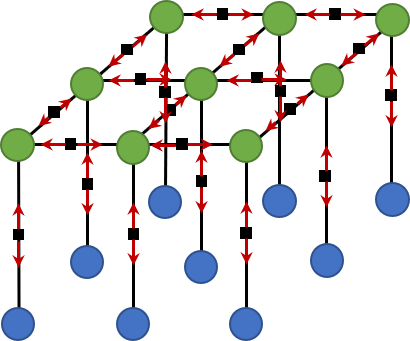
\includegraphics[width=\textwidth]{structured_prediction/factor_to_variable_msg.png}
    \caption{factor-to-variable-messages}
    \label{fig:factor_variable_msg}
  \end{subfigure}
  %
  \begin{subfigure}[h]{0.40\textwidth}
    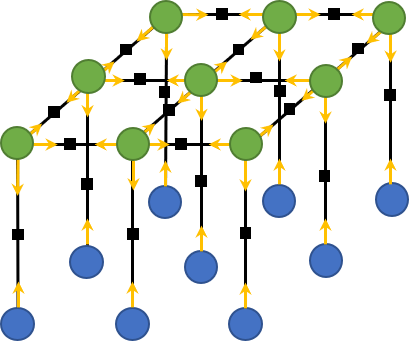
\includegraphics[width=\textwidth]{structured_prediction/variable_to_factor_msg.png}
    \caption{variable-to-factor messages}
    \label{fig:variable_factor_msg}
  \end{subfigure}
    \caption{Message passing algorithm on a factor graph created for an image of size $3\times 3$ pixels.}
    \label{fig:inference_msgs}
\end{figure}
After all messages are transferred, maximal beliefs for each factor are computed and a winning label is chosen, and the whole process is repeated in the next iteration. Inference is said to be completed when the state of convergence is achieved, which means when a change of maximal beliefs is smaller than a chosen convergence tolerance coefficient.

\newpage
Presented inference algorithms allow predicting the optimal configuration of labels for unclassified test samples given the observed data and an established model in a form of a factor graph. The model can be defined by expertise, however, usually it is trained based on known train samples by a machine learning process.